\chapter{Background} \label{ch:background}

Detailed description of many things. Blurb - brief description of cheminformatics, applications of computational tools to drug discovery. Maybe introduce design-make-teset? This stuff is probably in the introduction.

% \section{Molecular Transformer}
% The task in organic chemical reaction prediction is to predict the outcome (product or products) and potentially the yield of some organic reaction given the reactants, reagents, catalysts and conditions such as the solvent, temperature, reaction time etc.  This is both an academic and an industrial problem. It is of scientific interest to understand the different factors determining the outcome of reactions that are essential for the design of a successful reaction prediction model but it is also of interest for industry, in particular the pharmaceutical industry who wants to be able to synthesise drug candidate molecules quickly and efficiently to accelerate the drug discovery pipeline. There are several ways of tackling this problem all of them can be useful for different aspects of the prediction problem. \par

% \section{\emph{Ab-initio} reaction prediction}

% When trying to optimize certain reactions to find for example the best catalyst, a full modelling approach based on quantum mechanics is often used \cite{Shan2017PracticalApplications}. These methods can be very accurate, but their use is limited to expert theoreticians and relatively simple systems. If one wants to simulate reactions of larger systems an alternative can be the use of reactive force fields like ReaxFF \cite{Senftle2016TheDirections}. This approach relies on classical interatomic potentials which have the benefit of cheap evaluation but also allows bond breaking and forming unlike classical force fields which usually require pre-defined connectivity of the atoms. Another method often used to predict the selectivity of some particular type of reaction with high accuracy relies on properties of the reactants and reagents obtained using quantum chemical calculations. For example to determine the most probable reaction site in electrophilic aromatic substitution reaction the RegioSQM method finds the aromatic carbon with the lowest free energy of protonation. It is shown by the authors that this carbon is the most reactive site in over 96\% of the reactions considered in the paper \cite{Xu2014MechanismAlcohols}. Another notable example is the method developed by Cao et. al. which automates quantum chemical calculations at the density functional theory level and makes predictions based on them without requiring any expertise in computational methods \cite{Cao2020InReactions}.  They concentrate on Pd catalysed C - H activation reactions and determine the most probable outcome by automatically generating possible intermediate structures and using their energies as a proxy for the energy barrier of the reaction to proceed via the given route. \par

% \section{Rule-based reaction prediction}

% Often it is not necessary to fully simulate and understand a chemical reaction and it is sufficient to know the outcome i.e. the major product of it. This is most often the case when experimental organic chemists are willing to validate their synthetic route or when a synthesis planning software uses a reaction prediction model to score its suggestions. This is what is more traditionally referred to as reaction prediction. In these use cases a general purpose model that is able to predict a wide variety of organic reactions with good accuracy is desired. Trained organic chemists usually rationalize reactions based on the reaction mechanisms \cite{Clayden2012}. These mechanisms can be used to categorize organic reactions and each of these categories can be summarised with the help of so called reaction templates. Figure~\ref{fig:rx_template} shows a typical general reaction template for the synthesis of an amide using acid chloride and an amine. Here the $R_1$ and $R_2$ represent any chemical structures. 
% \begin{figure}[htbp!] 
% \centering    
% 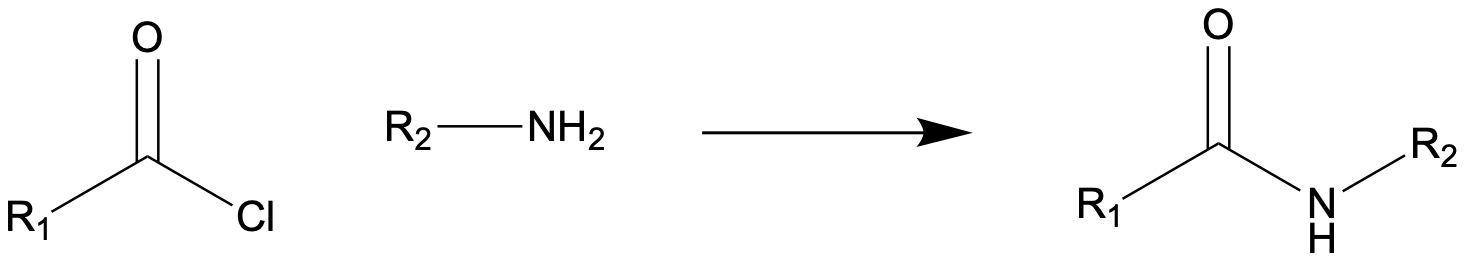
\includegraphics[width=0.75\textwidth]{Chapter2/Figs/Raster/rx_template.png}
% \caption[Reaction template]{An example of a reaction template for the synthesis of an amide}
% \label{fig:rx_template}
% \end{figure}
% These templates can be used for organic reaction prediction by building a catalogue of templates of as many organic reactions as possible. Then given some reactants and reagents as labelled graphs the problem of reaction prediction is transformed into one of subgraph searching to find the best matching general template in the catalogue. When that template is found it can be applied on the input to obtain the predicted outcome of the reaction. This approach was originally proposed and pioneered in the 1980s by E. J. Corey when he used templates for the reverse problem of retrosynthesis \cite{Corey1985Computer-assistedSynthesis}. The template-based approach had some success in forward reaction prediction for example as described in Ref~\cite{Klucznik2018EfficientLaboratory} a template-based model helped design synthetic pathways to a diverse set of 8 drug-like molecules. This method had considerably more success  in retrosynthesis though where there does not exist a single correct solution. One of the major limitation of template-based approaches when applied to forward prediction is scalability, meaning that the template library needs to be maintained and every time a new reaction is reported the associated template needs to be added to the template library. A further problem is that it is often not obvious which parts of the molecule are crucial for a given reaction. This means that given a reaction one can derive a smaller more general template or a larger one that is more specific for the particular reaction. This results in either too many templates matching a particular input resulting in many equally possible reaction outcomes or in the case of larger more specific templates the library will grow very big which results in very slow predictions.  \par

% \section{Data-driven reaction prediction}

% Modern approaches to reaction prediction increasingly rely on experimentally reported chemical reaction data instead of the knowledge of mechanisms. This can be advantageous for a number of reasons. The revolution of machine learning, pattern recognition and artificial intelligence resulted in a number of powerful methods developed in different fields such as natural language processing or graph generation that can be adapted for reaction prediction. These algorithms together with the several datasets containing hundreds of thousands or millions of reactions extracted from publications and patents using text mining have the potential for the development of successful models. These data driven models have the advantage that they can in principle build on all published reactions in the literature that no human chemist could look through to code up by hand. Furthermore, by learning from vast amount of data these machine learning models have the potential of learning complex chemical relationships resulting in better generalization. This is essential as the expectation for the reaction prediction models is to perform well on unseen molecules and potentially unseen reactions making them more than a simple searchable database. A limitation of these approaches is that the reaction databases often only contain the reactants and reagents and the major products, but not the minor products, yields, temperatures or other conditions. This makes the reaction prediction task an ill-posed problem. It is often the case that conditions such as temperature play a key role in determining the reaction outcome. For example in the case of enolate chemistry low temperature favours the formation of the kinetic, high temperature the thermodynamic enolate resulting in different selectivity \cite{Clayden2012}. Without specifying the temperature in these cases the major product cannot be determined. \par

% The first approach to data driven reaction prediction is very similar to the simple template based reaction prediction discussed above the only difference being that the templates are automatically extracted from the databases rather than being hand crafted \cite{Bgevig2015RoutePrediction, Kayala2012ReactionPredictor:Learning, Kayala2011LearningReactions,  Socorro2005ROBIA:Program}. This solves the issue of scalability but suffers from much of the same problems with the small templates being too general and large templates being too specific.  \par

% Machine learning models can also be used to directly predict the outcome of chemical reactions. These template-free approaches do not require any subgraph searching which results in much faster predictions. Another advantage is that since they are not directly memorizing templates from the training datasets they have the potential of better generalization by inferring some of the underlying reactivity trends. One of the first successful machine learning based model was proposed by Coley et. al. in 2017 \cite{Coley2017PredictionLearning}. Their approach builds on the template based models and combines them with neural networks. First a number of candidate products are generated using general templates extracted form the literature. These candidate templates are than scored using a neural network model trained to identify the major product. \par
% An improved model published by the same group has abandoned templates entirely \cite{ Coley2019AReactivity, Jin2017}. They have made use of the observation that usually only a small number of atoms and bonds participate directly in a chemical transformation. By considering the reactants and reagents as molecular graphs and the reaction as a series of graph edits they trained a reaction centre identifier network. This network selects a small number of atom pairs that are most likely to be involved in the reaction. All possible chemically valid graph edits are than considered on these centres. It is important to note that not all bond changes on the reaction centres have identical probabilities, and a product that results from more probable bond changes is itself more probable. This provides an initial ranking of the possible products. This generated ranking of products is then refined by a Weisfeiler-Lehman Difference Network, a type of graph convolutional neural network, to find the most probable product structure.  Together with the model they have also published a dataset of ca 480 000 reactions filtered from the text mining work of Lowe \cite{Lowe2012}. They have achieved 85\% accuracy on this dataset outperforming the previous state-of-the-art by more than 10\%. The key strength of this approach is that interpretability is built into the design of the algorithm. The way the model is predicting the sequence of graph edits is very similar to how humans would write arrow-pushing mechanisms of organic reactions\cite{Clayden2012}. This way one can get a direct insight into how the model is arriving at certain predictions. This is in contrast to previous reaction prediction approaches that were trying to directly learn mechanisms based on expert crafted rules as a supervised learning problem \cite{Bradshaw2019APaths, Kayala2012ReactionPredictor:Learning}.  \par

\section{Molecular Representation}

\subsection{SMILES}
In the 2010s natural language processing (NLP) and neural machine translation saw a huge revolution \cite{Young2018RecentProcessing}. This led scientists from different fields to the realization that many problems can be cast in a sequence-to-sequence formalism. This allowed them to use the powerful tools of NLP in a variety of applications. The first attempt to formulate the reaction prediction problem in a sequence-to-sequence manner came by Nam and Kim \cite{Nam2016LinkingReactions}. They have used a text based representation of organic molecules called SMILES \cite{Weininger1988, Weininger1989}. SMILES strings represent atoms with their chemical symbols and aromatic atoms with lowercase letters. Single and aromatic bonds are omitted while for double and triple bonds the specials characters \texttt{=} and \texttt{\#} are used. Branches are specified by enclosing them into parentheses. To encode cyclic structures a single bond in the ring is broken and the matching atoms are denoted by numbers. These rules lead to a large number of valid SMILES representations for larger molecules. To make the mapping injective a deterministic algorithm is used to enumerate the nodes of the molecular graph. Following this ordering a unique canonical text representation of organic molecules is obtained. This representation forms the basis for all of the text-based models discussed later. 
A few examples of the SMILES syntax with the corresponding structures is shown below. 

\begin{table}[!h]
\begin{center}
    \begin{tabular}{|c|c|}
    \hline
         SMILES & Structure \\
         \hline
         C & CH\textsubscript{4} \\
         \lbrack Fe2+\rbrack & Fe\textsuperscript{2+} \\
         C=O & CH\textsubscript{2}O \\
         C\#N & HCN (cyan) \\
         CCN(CC)CC & 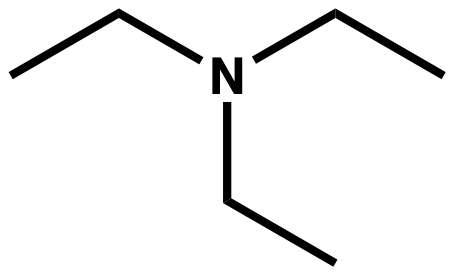
\includegraphics[width=0.75in]{Chapters/Background/Figs/triethyl_amine.png} \\
         CC1=CC(CCC1)Br & 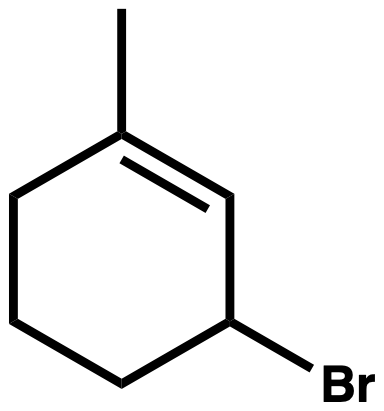
\includegraphics[width=0.7in]{Chapters/Background/Figs/cyclic.png} \\
         \hline
    \end{tabular}
    \caption{Demonstration of the SMILES language}
    \label{table:smiles}
\end{center}
\end{table}


\begin{figure}[!h]
    \centering
    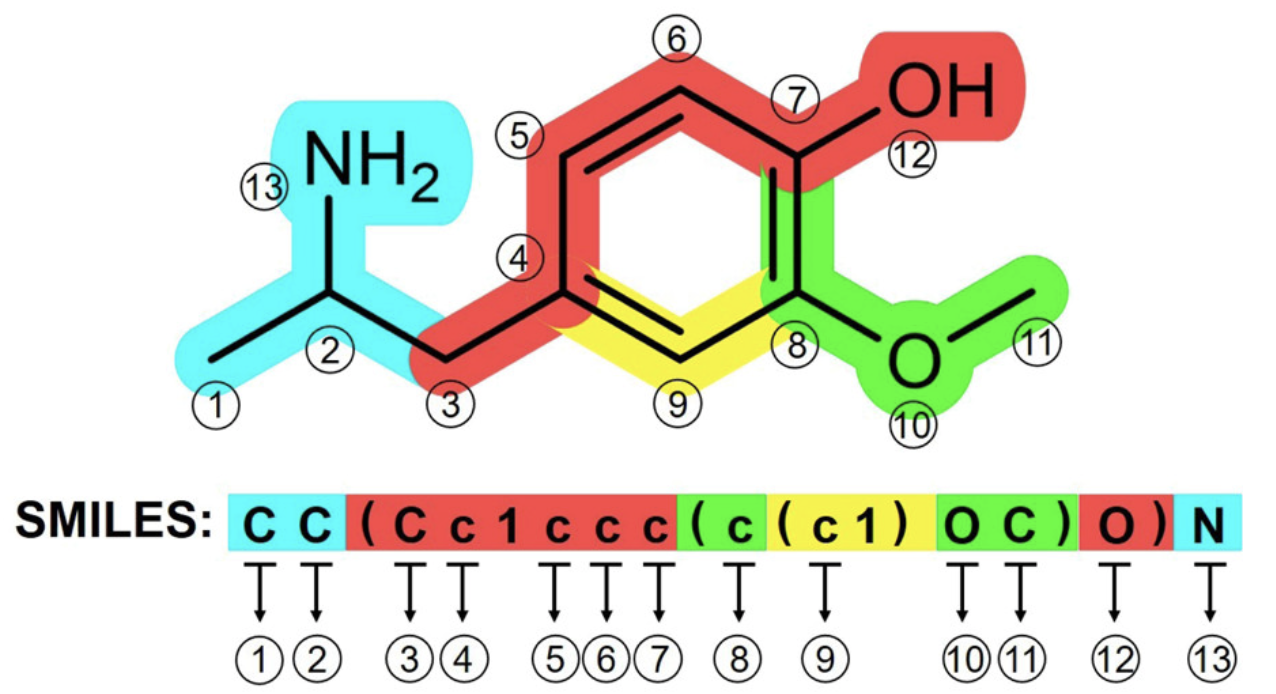
\includegraphics[width=0.8\textwidth]{Chapters/Background/Figs/smiles.png}
    \caption{\label{fig:smiles} \textbf{Illustration of the mapping from chemical structure to SMILES.} Adapted from \cite{Kim2021GenerativeCT}.}
\end{figure}

\subsection{SMARTS}

SMILES arbitrary target specification (SMARTS) is a language for specifying substructural patterns in molecules. The SMARTS line notation is expressive and allows extremely precise and transparent substructural specification and atom typing. % TODO - from wikipedia, update

%TODO - example table of SMARTS patterns


Chemical substructures. Scaffolds. Reaction templates.

%TODO - example applications from wikidia
The precise and transparent substructural specification that SMARTS allows has been exploited in a number of applications.

Substructural filters defined in SMARTS have been used [7] to identify undesirable compounds when performing strategic pooling of compounds for high-throughput screening. The REOS (rapid elimination of swill) [8] procedure uses SMARTS to filter out reactive, toxic and otherwise undesirable moieties from databases of chemical structures.

RECAP [9](Retrosynthetic Combinatorial Analysis Procedure) uses SMARTS to define bond types. RECAP is a molecule editor which generates fragments of structures by breaking bonds of defined types and the original link points in these are specified using isotopic labels. Searching databases of biologically active compounds for occurrences of fragments allows privileged structural motifs to be identified. The Molecular Slicer [10] is similar to RECAP and has been used to identify fragments that are commonly found in marketed oral drugs.

The Leatherface program[11] is a general purpose molecule editor which allows automated modification of a number of substructural features of molecules in databases, including protonation state, hydrogen count, formal charge, isotopic weight and bond order. The molecular editing rules used by Leatherface are defined in SMARTS. Leatherface can be used to standardise tautomeric and ionization states and to set and enumerate these in preparation of databases[12] for virtual screening. Leatherface has been used in Matched molecular pair analysis, which enables the effects of structural changes (e.g. substitution of hydrogen with chlorine) to be quantified,[13] over a range of structural types.
ALADDIN[14] is a pharmacophore matching program that uses SMARTS to define recognition points (e.g. neutral hydrogen bond acceptor) of pharmacophores. A key problem in pharmacophore matching is that functional groups that are likely to be ionised at physiological pH are typically registered in their neutral forms in structural databases. The ROCS shape matching program allows atom types to be defined using SMARTS.[15]

\subsection{Pharmacophores}

A pharmacophore is an abstract description of molecular features that are necessary for molecular recognition of a ligand by a biological macromolecule. IUPAC defines a pharmacophore to be "an ensemble of steric and electronic features that is necessary to ensure the optimal supramolecular interactions with a specific biological target and to trigger (or block) its biological response".[1] A pharmacophore model explains how structurally diverse ligands can bind to a common receptor site. Furthermore, pharmacophore models can be used to identify through de novo design or virtual screening novel ligands that will bind to the same receptor.

Typical pharmacophore features include hydrophobic centroids, aromatic rings, hydrogen bond acceptors or donors, cations, and anions. These pharmacophoric points may be located on the ligand itself or may be projected points presumed to be located in the receptor.

In modern computational chemistry, pharmacophores are used to define the essential features of one or more molecules with the same biological activity. A database of diverse chemical compounds can then be searched for more molecules which share the same features arranged in the same relative orientation. Pharmacophores are also used as the starting point for developing 3D-QSAR models. Such tools and a related concept of "privileged structures", which are "defined as molecular frameworks which are able of providing useful ligands for more than one type of receptor or enzyme target by judicious structural modifications",[3] aid in drug discovery.[4]

Use SMARTS to define pharmacophores.
\subsection{Fingerprints}

The similarity-based[4] virtual screening (a kind of ligand-based virtual screening) assumes that all compounds in a database that are similar to a query compound have similar biological activity. Although this hypothesis is not always valid,[5] quite often the set of retrieved compounds is considerably enriched with actives.[6] To achieve high efficacy of similarity-based screening of databases containing millions of compounds, molecular structures are usually represented by molecular screens (structural keys) or by fixed-size or variable-size molecular fingerprints. Molecular screens and fingerprints can contain both 2D- and 3D-information. However, the 2D-fingerprints, which are a kind of binary fragment descriptors, dominate in this area. Fragment-based structural keys, like MDL keys,[7] are sufficiently good for handling small and medium-sized chemical databases, whereas processing of large databases is performed with fingerprints having much higher information density. Fragment-based Daylight,[8] BCI,[9] and UNITY 2D (Tripos[10]) fingerprints are the best known examples. The most popular similarity measure for comparing chemical structures represented by means of fingerprints is the Tanimoto (or Jaccard) coefficient T. Two structures are usually considered similar if T > 0.85 (for Daylight fingerprints). However, it is a common misunderstanding that a similarity of T > 0.85 reflects similar bioactivities in general ("the 0.85 myth").[11]

Tanimoto similarity.

\section{Computational Approaches}

\subsection{Docking}

In the field of molecular modeling, docking is a method which predicts the preferred orientation of one molecule to a second when a ligand and a target are bound to each other to form a stable complex.[1] Knowledge of the preferred orientation in turn may be used to predict the strength of association or binding affinity between two molecules using, for example, scoring functions.

Schematic illustration of docking a small molecule ligand (green) to a protein target (black) producing a stable complex.
0:13
Docking of a small molecule (green) into the crystal structure of the beta-2 adrenergic G-protein coupled receptor (PDB: 3SN6)
The associations between biologically relevant molecules such as proteins, peptides, nucleic acids, carbohydrates, and lipids play a central role in signal transduction. Furthermore, the relative orientation of the two interacting partners may affect the type of signal produced (e.g., agonism vs antagonism). Therefore, docking is useful for predicting both the strength and type of signal produced.
Molecular docking is one of the most frequently used methods in structure-based drug design, due to its ability to predict the binding-conformation of small molecule ligands to the appropriate target binding site. Characterisation of the binding behaviour plays an important role in rational design of drugs as well as to elucidate fundamental biochemical processes.[2][3]

One can think of molecular docking as a problem of “lock-and-key”, in which one wants to find the correct relative orientation of the “key” which will open up the “lock” (where on the surface of the lock is the key hole, which direction to turn the key after it is inserted, etc.). Here, the protein can be thought of as the “lock” and the ligand can be thought of as a “key”. Molecular docking may be defined as an optimization problem, which would describe the “best-fit” orientation of a ligand that binds to a particular protein of interest. However, since both the ligand and the protein are flexible, a “hand-in-glove” analogy is more appropriate than “lock-and-key”.[4] During the course of the docking process, the ligand and the protein adjust their conformation to achieve an overall "best-fit" and this kind of conformational adjustment resulting in the overall binding is referred to as "induced-fit".[5]
Molecular docking research focuses on computationally simulating the molecular recognition process. It aims to achieve an optimized conformation for both the protein and ligand and relative orientation between protein and ligand such that the free energy of the overall system is minimized.

To perform a docking screen, the first requirement is a structure of the protein of interest. Usually the structure has been determined using a biophysical technique such as X-ray crystallography, NMR spectroscopy or cryo-electron microscopy (cryo-EM), but can also derive from homology modeling construction. This protein structure and a database of potential ligands serve as inputs to a docking program. The success of a docking program depends on two components: the search algorithm and the scoring function.
Search algorithm[edit]
Main article: Searching the conformational space for docking
The search space in theory consists of all possible orientations and conformations of the protein paired with the ligand. However, in practice with current computational resources, it is impossible to exhaustively explore the search space — this would involve enumerating all possible distortions of each molecule (molecules are dynamic and exist in an ensemble of conformational states) and all possible rotational and translational orientations of the ligand relative to the protein at a given level of granularity. Most docking programs in use account for the whole conformational space of the ligand (flexible ligand), and several attempt to model a flexible protein receptor. Each "snapshot" of the pair is referred to as a pose.
A variety of conformational search strategies have been applied to the ligand and to the receptor. These include:
systematic or stochastic torsional searches about rotatable bonds
molecular dynamics simulations
genetic algorithms to "evolve" new low energy conformations and where the score of each pose acts as the fitness function used to select individuals for the next iteration.

Ligand flexibility[edit]
Conformations of the ligand may be generated in the absence of the receptor and subsequently docked[14] or conformations may be generated on-the-fly in the presence of the receptor binding cavity,[15] or with full rotational flexibility of every dihedral angle using fragment based docking.[16] Force field energy evaluation are most often used to select energetically reasonable conformations,[17] but knowledge-based methods have also been used.[18]
Peptides are both highly flexible and relatively large-sized molecules, which makes modeling their flexibility a challenging task. A number of methods were developed to allow for efficient modeling of flexibility of peptides during protein-peptide docking.[19]
Receptor flexibility[edit]
Computational capacity has increased dramatically over the last decade making possible the use of more sophisticated and computationally intensive methods in computer-assisted drug design. However, dealing with receptor flexibility in docking methodologies is still a thorny issue.[20] The main reason behind this difficulty is the large number of degrees of freedom that have to be considered in this kind of calculations. Neglecting it, however, in some of the cases may lead to poor docking results in terms of binding pose prediction.[21]
Multiple static structures experimentally determined for the same protein in different conformations are often used to emulate receptor flexibility.[22] Alternatively rotamer libraries of amino acid side chains that surround the binding cavity may be searched to generate alternate but energetically reasonable protein conformations.[23][24]
Scoring function[edit]
Main article: Scoring functions for docking
Docking programs generate a large number of potential ligand poses, of which some can be immediately rejected due to clashes with the protein. The remainder are evaluated using some scoring function, which takes a pose as input and returns a number indicating the likelihood that the pose represents a favorable binding interaction and ranks one ligand relative to another.
Most scoring functions are physics-based molecular mechanics force fields that estimate the energy of the pose within the binding site. The various contributions to binding can be written as an additive equation:

% {\displaystyle \bigtriangleup G_{bind}=\bigtriangleup G_{solvent}+\bigtriangleup G_{conf}+\bigtriangleup G_{int}+\bigtriangleup G_{rot}+\bigtriangleup G_{t/t}+\bigtriangleup G_{vib}}
The components consist of solvent effects, conformational changes in the protein and ligand, free energy due to protein-ligand interactions, internal rotations, association energy of ligand and receptor to form a single complex and free energy due to changes in vibrational modes.[25] A low (negative) energy indicates a stable system and thus a likely binding interaction.
Alternative approaches use modified scoring functions to include constraints based on known key protein-ligand interactions,[26] or knowledge-based potentials derived from interactions observed in large databases of protein-ligand structures (e.g. the Protein Data Bank).[27]
There are a large number of structures from X-ray crystallography for complexes between proteins and high affinity ligands, but comparatively fewer for low affinity ligands as the latter complexes tend to be less stable and therefore more difficult to crystallize. Scoring functions trained with this data can dock high affinity ligands correctly, but they will also give plausible docked conformations for ligands that do not bind. This gives a large number of false positive hits, i.e., ligands predicted to bind to the protein that actually don't when placed together in a test tube.
One way to reduce the number of false positives is to recalculate the energy of the top scoring poses using (potentially) more accurate but computationally more intensive techniques such as Generalized Born or Poisson-Boltzmann methods.[9]

Simulating the docking process is much more complicated. In this approach, the protein and the ligand are separated by some physical distance, and the ligand finds its position into the protein's active site after a certain number of “moves” in its conformational space. The moves incorporate rigid body transformations such as translations and rotations, as well as internal changes to the ligand's structure including torsion angle rotations. Each of these moves in the conformation space of the ligand induces a total energetic cost of the system. Hence, the system's total energy is calculated after every move.
The obvious advantage of docking simulation is that ligand flexibility is easily incorporated, whereas shape complementarity techniques must use ingenious methods to incorporate flexibility in ligands. Also, it more accurately models reality, whereas shape complementary techniques are more of an abstraction.
Clearly, simulation is computationally expensive, having to explore a large energy landscape. Grid-based techniques, optimization methods, and increased computer speed have made docking simulation more realistic.

Docking assessment[edit]
See also: Critical Assessment of Prediction of Interactions
The interdependence between sampling and scoring function affects the docking capability in predicting plausible poses or binding affinities for novel compounds. Thus, an assessment of a docking protocol is generally required (when experimental data is available) to determine its predictive capability. Docking assessment can be performed using different strategies, such as:
docking accuracy (DA) calculation;
the correlation between a docking score and the experimental response or determination of the enrichment factor (EF);[28]
the distance between an ion-binding moiety and the ion in the active site;
the presence of induce-fit models.
Docking accuracy[edit]
Docking accuracy[29][30] represents one measure to quantify the fitness of a docking program by rationalizing the ability to predict the right pose of a ligand with respect to that experimentally observed.[31]
Enrichment factor[edit]
Docking screens can also be evaluated by the enrichment of annotated ligands of known binders from among a large database of presumed non-binding, “decoy” molecules.[28] In this way, the success of a docking screen is evaluated by its capacity to enrich the small number of known active compounds in the top ranks of a screen from among a much greater number of decoy molecules in the database. The area under the receiver operating characteristic (ROC) curve is widely used to evaluate its performance.
Prospective[edit]
Resulting hits from docking screens are subjected to pharmacological validation (e.g. IC50, affinity or potency measurements). Only prospective studies constitute conclusive proof of the suitability of a technique for a particular target.[32] In the case of G protein-coupled receptors (GPCRs), which are targets of more than 30% of marketed drugs, molecular docking led to the discovery of more than 500 GPCR ligands.[33]
Benchmarking[edit]
The potential of docking programs to reproduce binding modes as determined by X-ray crystallography can be assessed by a range of docking benchmark sets.
For small molecules, several benchmark data sets for docking and virtual screening exist e.g. Astex Diverse Set consisting of high quality protein-ligand X-ray crystal structures[34] or the Directory of Useful Decoys (DUD) for evaluation of virtual screening performance.[28]
An evaluation of docking programs for their potential to reproduce peptide binding modes can be assessed by Lessons for Efficiency Assessment of Docking and Scoring (LEADS-PEP).[35]
Applications[edit]
A binding interaction between a small molecule ligand and an enzyme protein may result in activation or inhibition of the enzyme. If the protein is a receptor, ligand binding may result in agonism or antagonism. Docking is most commonly used in the field of drug design — most drugs are small organic molecules, and docking may be applied to:
hit identification – docking combined with a scoring function can be used to quickly screen large databases of potential drugs in silico to identify molecules that are likely to bind to protein target of interest (see virtual screening). Reverse pharmacology routinely uses docking for target identification.
lead optimization – docking can be used to predict in where and in which relative orientation a ligand binds to a protein (also referred to as the binding mode or pose). This information may in turn be used to design more potent and selective analogs.
bioremediation – protein ligand docking can also be used to predict pollutants that can be degraded by enzymes.[36][37]

Theory. Virtual screening. Virtual library?

In contrast to high-throughput screening, virtual screening involves computationally screening in silico libraries of compounds, by means of various methods such as docking, to identify members likely to possess desired properties such as biological activity against a given target. In some cases, combinatorial chemistry is used in the development of the library to increase the efficiency in mining the chemical space. More commonly, a diverse library of small molecules or natural products is screened.

\subsection{FEP?}

\section{Machine Learning}

\subsection{Random Forest}

Random forests or random decision forests is an ensemble learning method for classification, regression and other tasks that operates by constructing a multitude of decision trees at training time. For classification tasks, the output of the random forest is the class selected by most trees. For regression tasks, the mean or average prediction of the individual trees is returned.[1][2] Random decision forests correct for decision trees' habit of overfitting to their training set.[3]:587–588 Random forests generally outperform decision trees, but their accuracy is lower than gradient boosted trees.[citation needed] However, data characteristics can affect their performance.[4][5]

Random Forests are a decision tree-based model that use an ensemble of multiple weak regressors to make predictions [47]. Each tree is constructed to find a series of decision boundaries that split the data to minimise the squared deviations between the samples and the sample mean in each branch or leaf of the tree. Predictions are made by averaging the outputs of the different trees when applied to new data. To overcome issues of over-fitting common to decision tree methods, Random Forests use bagging and random subspace projection to reduce the correlation between the trees, improving their generalisation performance.

Examples of RF with morgan fingerprints.
\subsection{Deep Learning}

In contrast to shallow learning, the deep learning revolution of the last decade is built around models that learn their representations from raw data inputs. The workhorse of deep learning is the neural network. At their heart, neural networks are compositions of feature maps that transform the raw input features, x, into a new set of features that are linearly related to their target, y. The prototypical example of a neural network is the multi-layer perceptron (MLP). A l-layer MLP approximates functions f(x) using l successive non-linear feature maps constructed as compositions of affine transformations and non linearities, i.e.

Neural Networks. Loss functions. Optimisation.

\begin{equation}
    y = f(x, \theta)
\end{equation}

\begin{equation}
    \hat{theta} = \arg\min_{\theta} \mathcal{L}(\theta)
\end{equation}

\begin{equation}
    \hat{y} = \sigma(\mathbf{W} \cdot \mathbf{x} + \mathbf{b})
\end{equation}

\begin{equation}
    \mathcal{L}(y, \hat{y}) = \sum_{i}(y_i - \hat{y}_i)^{2}
\end{equation}

The remarkable success of deep learning emerges from the fact that neural networks, such as MLPs, can be optimised effectively using first-order gradient-based approaches. Moreover, the necessary gradients can be efficiently calculated using the chain rule by back- propagation of the training loss. In practice, modern neural networks are implemented inside automatic differentiation frameworks that abstract away the technical burden of implementing back-propagation [71, 72]. In addition, these frameworks are designed to enable the necessary calculations to be carried out on hardware accelerators, such as graphical processing units (GPUs), that dramatically reduce the time for training.
The most simple gradient-based optimisation algorithm is gradient-descent. In gradient descent at each step the model’s parameters are updated according to

\begin{equation}
    \theta_{t+1} = \theta_t - \eta \nabla_{\theta} \mathcal{L}
\end{equation}

where the learning rate, $\eta$, is a hyper-parameter of the optimiser that determines the size of the parameter updates. In practice, the full-batch gradient of the loss, $\nabla_{\theta}\mathcal{L}(\theta_{t})$ is replaced with a stochastic approximation of the gradient calculated on a mini-batch of data randomly sampled from all the available training data. Typically mini-batches are randomly drawn from the training data without replacement until all the training examples have been considered. Each complete cycle through the training set is referred to as an epoch. After each epoch, the training set is shuffled and the process is repeated until the loss has satisfactorily converged. Replacing full-batch gradient descent with mini-batch stochastic gradient descent significantly speeds up optimisation, reducing the amount of computation required to determine the gradient for each step and providing helpful regularisation effects that drive the optimisation towards flatter local basins of attraction in the loss landscape. Further improvements to model optimisation procedures can be achieved by incorporating additional terms such as momentum, learning rate schedules, or adaptive learning rates [73], and additional regularisation procedures such as weight decay, early-stopping, or dropout [74].

In the above description of the MLP, the key requirement is that the model is end- to-end differentiable. This allows the parameters of the model to be optimised by the combination of back-propagation and gradient descent. Accordingly, provided we ensure that all operations in our models have defined derivatives, we can build up novel neural networks architectures with specific inductive biases as compositions of custom differentiable building blocks – notable examples are recurrent neural networks (RNNs) that are designed to handle series data (e.g. Gated-Recurrent-Unit (GRU) [75] and Long-Short-Term-Memory (LSTM) networks [76]) and convolutional neural networks
(CNNs) that build in translational invariance for computer vision applications (e.g. LeNet [77], AlexNet [78], and ResNets [79]).

Within materials science, this ability to compose differentiable building blocks into novel architectures has led to the development of a wide variety of message-passing neural networks that operate directly on the atomic coordinates of molecules and materials. Typically these models operate on “radius”-graphs of interconnected local environments determined using a cutoff radius – the resulting data structure closely mirrors that of Verlet lists used in atomistic simulations [80]. The nodes of the graphs encode atoms with edges encoding interactions or bonds. As with shallow descriptor-based models, it is important to encode the underlying symmetries of the problem into the network architecture. Earlier models ensured SO(3)-invariance by only including position information via the relative distances between connected sites [81–83]. More recently SO(3)-equivariant architectures have been proposed that include angular and higher-order information or relative displacement vectors between atoms to allow construction of message passing operations that maintain equivariance [84].



Examples of NNs with fingerprints and SMILES.

\subsection{Evaluating Models}

ROC-AUC. Accuracy. Enrichment.

%TODO - from wikipedia
A receiver operating characteristic curve, or ROC curve, is a graphical plot that illustrates the diagnostic ability of a binary classifier system as its discrimination threshold is varied.

The ROC curve is created by plotting the true positive rate (TPR) against the false positive rate (FPR) at various threshold settings. The true-positive rate is also known as sensitivity, recall or probability of detection.[10] The false-positive rate is also known as probability of false alarm[10] and can be calculated as (1 - specificity).

\begin{equation}
    \mathrm{EF}(n) = \frac{\mathrm{Hit\: rate (predicted\: top - }n)}{\mathrm{Hit\: rate (baseline)}}
\end{equation}


Train-Test splitting

Random split, scaffold split, time split

In machine learning, a common task is the study and construction of algorithms that can learn from and make predictions on data.[1] Such algorithms function by making data-driven predictions or decisions,[2] through building a mathematical model from input data. These input data used to build the model are usually divided in multiple data sets. In particular, three data sets are commonly used in different stages of the creation of the model: training, validation and test sets.
The model is initially fit on a training data set,[3] which is a set of examples used to fit the parameters (e.g. weights of connections between neurons in artificial neural networks) of the model.[4] The model (e.g. a naive Bayes classifier) is trained on the training data set using a supervised learning method, for example using optimization methods such as gradient descent or stochastic gradient descent. In practice, the training data set often consists of pairs of an input vector (or scalar) and the corresponding output vector (or scalar), where the answer key is commonly denoted as the target (or label). The current model is run with the training data set and produces a result, which is then compared with the target, for each input vector in the training data set. Based on the result of the comparison and the specific learning algorithm being used, the parameters of the model are adjusted. The model fitting can include both variable selection and parameter estimation.
Successively, the fitted model is used to predict the responses for the observations in a second data set called the validation data set.[3] The validation data set provides an unbiased evaluation of a model fit on the training data set while tuning the model's hyperparameters[5] (e.g. the number of hidden units—layers and layer widths—in a neural network[4]). Validation datasets can be used for regularization by early stopping (stopping training when the error on the validation data set increases, as this is a sign of over-fitting to the training data set).[6] This simple procedure is complicated in practice by the fact that the validation dataset's error may fluctuate during training, producing multiple local minima. This complication has led to the creation of many ad-hoc rules for deciding when over-fitting has truly begun.[6]
Finally, the test data set is a data set used to provide an unbiased evaluation of a final model fit on the training data set.[5] If the data in the test data set has never been used in training (for example in cross-validation), the test data set is also called a holdout data set. The term "validation set" is sometimes used instead of "test set" in some literature (e.g., if the original data set was partitioned into only two subsets, the test set might be referred to as the validation set).[5]
Deciding the sizes and strategies for data set division in training, test and validation sets is very dependent on the problem and data available.[7]

Note on bioactivity?

% In the paper of Nam and Kim they formulated the reaction prediction problem as a translation task. The input SMILES corresponding to the reactant and reagent molecules are tokenized, so that each character of SMILES is equivalent to a word and the whole input is equivalent to a sentence. This sentence is than ``translated" by the model to the product SMILES. Neural machine translation models are trained using a large parallel corpus. This is available in the case of organic reactions from patents and publications or can be generated using templates of elementary reactions. The method of Nam and Kim served as an important proof of concept but could not match the accuracy of rule-based and graph-to-graph models. \par
% %The method was built on a neural network building block called gated recurrent unit (GRU) \cite{Cho2014LearningTranslation}. GRUs are a type of recurrent neural networks that process arbitrarily long inputs token by token, so that the hidden state representation of each token depends on the previous ones. %The model used in the paper is illustrated on Figure~\ref{fig:gru}. 
% %This model served as a proof-of-concept but could not match the accuracy of graph-to-graph and template based approaches. \par

% \iffalse
% \begin{figure}[htbp!] 
% \centering    
% \includegraphics[width=0.9\textwidth]{Chapter2/Figs/Raster/gru.png}
% \caption[GRU for reaction predictions]{The architecture used by Nam and Kim. The input SMILES string is tokenized into ``words", each token is embedded using a learnt embedding and processed by a three layer GRU network. The product is generated using attention mechanism.}
% \label{fig:gru}
% \end{figure}
% \fi

% The large breakthrough of sequence-to-sequence models for reaction prediction came after the introduction of a new and innovative architecture for neural machine translation by Vaswani et. al. \cite{Vaswani2017}. The so called Transformer model revolutionized the entire industry of machine translation and found use in many other areas of machine learning ever since. In the next section the Transformer architecture is described in detail followed by a discussion of the Molecular Transformer. 

% \section{The Molecular Transformer}

% \subsection{The Transformer architecture}

% The Transformer architecture was originally developed for machine translation tasks. It has an encoder-decoder structure. Both the encoder and the decoder are made up of so called transformer blocks that process the inputs by applying a multi-head scaled dot-product attention mechanism followed by layer normalization and some fully connected feed forward layers. In the following each part is described in detail. 

% \subsubsection{Encoder}
% The input to the model is a sentence made up of different words that are contained in a vocabulary. Each word in the vocabulary has a learnt fixed-length vector representation. Passing these vectors to the model would not be enough though as these vectors have no reference to where the given word appears inside the sequence. To encode this information as well another vector of the same length is added to each word-vector that depends on the position inside the sequence: \par

% \begin{equation}
%     PE_{(pos, 2i)}=\sin(pos/10000^{2i/d_{model}})
% \end{equation}
% \begin{equation}
%     PE_{(pos, 2i+1)}=\cos(pos/10000^{2i/d_{model}})
% \end{equation}

% This vector representation of the input text is passed into the transformer blocks. These consist of a multi-head attention layer with residual connection \cite{He2016DeepRecognition} followed by layer normalization \cite{Ba2016LayerNormalization} and a 2-layer fully connected feed forward neural network with ReLU activation. The encoder of the model is made up of $N=6$ transformer blocks as illustrated on Figure~\ref{fig:transformer}

% \begin{figure}[ht]
% \centering    
% \includegraphics[width=2.9in]{transformer_diagram.png}
% \caption{Graphical illustration of the full transformer model \cite{Vaswani2017}}
% \label{fig:transformer}
% \end{figure}

% \subsubsection{Multi-head scaled dot-product attention}
% The multi-head scaled dot-product attention is the heart of the Transformer model. It is a specific version of a general deep learning technique called attention. Given a set of vector \emph{values} and a vector \emph{query} the attention mechanism computes a weighted sum of the \emph{values} dependent on the \emph{query}. The sum represents a selective summary of the \emph{values} and the \emph{query} determines the importance of each vector, i. e. determines how much each \emph{value} vector is attended to.\par 
% The full attention mechanism operates by performing the following steps. Given some vector values $\bm{h_1}, \bm{h_2},\dots, \bm{h_N} \in \mathbb{R} ^{d_1}$ and a query $\bm{q} \in \mathbb{R} ^{d_2}$ \par

% \begin{enumerate}
%     \item First the attention scores $\bm{e} \in \mathbb{R}^N$ are computed. In the case of the scaled dot-product attention $d_1=d_2$ and $\bm{e}$ is simply defined as the scaled vector of projections $e_i=\frac{\bm{q}^\intercal \bm{h}_i}{\sqrt{d_1}}$
%     \item To generate the attention distribution $\bm{\alpha}$ the softmax of $\bm{e}$ is taken: 
%     \begin{equation}
%         \alpha_i=\frac{\exp{(e_i)}}{\sum_{j=1}^N \exp{(e_j)}} 
%         \label{eqn:softmax}
%     \end{equation}
%     \item Finally the attention distribution is used to take the weighted sum of the values to obtain the final output
%     \begin{equation}
%         \bm{a}=\sum_{i=1}^N \alpha_i \: \bm{h}_i \; \in \mathbb{R}^{d_1}
%     \end{equation}
% \end{enumerate}

% The scaling factor in the dot product serves the purpose of preventing some of the projection becoming overwhelmingly large which in turn would lead to the softmax function being sharply peaked around those values and being shallow everywhere else. This would result in very small gradients at most places that can substantially slow down the training.\par

% In the Transformer encoder the above described attention mechanism is used such that given a set of input vectors a new vector is calculated for all of them (being the query) from the others (being the keys). This is called self-attention. This way during training the model is able to learn which vectors (that are representing words or atoms) usually interact with each other. This interaction can result in a large value in the attention distribution. \par

% Usually the input, be it a chemical formula or a sentence contains a rich structure with the words affecting each others meanings in multiple ways. The problem with the simple self-attention mechanism is that by defining a single attention distribution for each input vector only one way of interaction can be learnt by the model. To give the model more flexibility to potentially learn more complex interaction structures multi-head attention was introduced. This mechanism maps the vectors to $h=8$ different lower dimensional spaces via a set of learnt linear transformations. The self-attention mechanism is than applied in these lower dimensional spaces simultaneously. The outputs of the different attention heads are finally concatenated and fed into a linear neural network layer. The whole mechanism is illustrated on Figure~\ref{fig:multihead_attention}

% \begin{figure}
% \centering    
% \includegraphics[width=2.2in]{mulithead_attention.png}
% \caption{Graphical illustration of the multi-head attention \cite{Vaswani2017}}
% \label{fig:multihead_attention}
% \end{figure}

% \subsubsection{Decoder}

% The outputs of the encoder which are $N$ vectors if the input sequence is $N$ words long are fed into the decoder which has a structure almost identical to the encoder. The first modifications concern the masking in the multi-head self-attention layers to make sure that every token in the output translation can only attend to the preceding ones. The second modification of the attention mechanism is making use of the encoder outputs by using them as keys whilst the queries are the outputs of the previous decoder layer. \par
% The generation of the translation happens in a sequential manner. First the embedding of the special \texttt{<start>} token is fed into the decoder and passed through the layers. The result is projected to a vector that has the same dimensionality as the size of the vocabulary. Finally the softmax function is applied to obtain the probability of the first word. The second word is generated by passing in the first word (and the \texttt{start} token) to the decoder, the third is generated by passing in the first and the second etc. This is called autoregressive translation. Finally the translation terminates either when the most probable next token is the special \texttt{<end>} token or when the maximum sequence length is reached. By multiplying together the next-token probabilities and normalizing with respect to the length of the output a confidence score of the translation can be obtained. 


% \subsubsection{Datasets}
% The first dataset used in this work is the freely available USPTO dataset \cite{Lowe2012} that was filtered by Jin et. al. \cite{Jin2017}. Further filtering was preformed to remove some remaining duplicates or reactions that were erroneously text mined. These included examples such as reactions whose sole product is nitric acid, sulfuric acid, chloride ion etc. This way the final number of reactions in the dataset was 471 791 of which 377 419  were used for training, 23 589 for validation and 70 765 were used as a hold-out test set. The training set was augmented by an equal number of random equivalent SMILES strings. Augmentation can help the model to learn the underlying molecular graph from the SMILES sequence. \par
% The model trained in the way described above achieved 88.8\% Top-1 accuracy on the test set. This model was used throughout the interpretability experiments and is referred to as USPTO Transformer. \par
% The second dataset used was the commercial Pistachio dataset \cite{Mayfield2018Pistachio2.0}. This dataset contains over 9 million reactions text mined from US and EPO patents. This dataset was filtered similarly to USPTO to remove erroneous and duplicate reactions. It turned out that many of the 9 million reactions were duplicates corresponding to different patent IDs. In the end a dataset of 2 375 385 reactions was obtained of which 2 019 078 was used for training, 118 770 for validation and 237 537 for testing. \par
% The model trained as described above achieved 76.4\% Top-1 accuracy on the test set. Even though this looks like a substantially lower performance in reality the two models perform similarly well on new reactions. The possible reasons for the large difference in the measured performance on the held-out test sets are described in detail in Chapter~\ref{chap:interpr_molt}. This model obtained was also used in the interpretability experiments to test the effect of increased training set size on the models understanding of chemistry and is referred to as Pistachio Transformer in the rest of the thesis. \par

% \subsection{Interpretability}
% Modern machine learning and especially deep learning algorithms are often regarded as black box machines. It is thought that the more complex a learning algorithm is the better it can fit complex pattern in the data, but it comes at the expense of human interpretability. This is a criticism that is present especially in scientific applications where the goal is not only to have a predictive model, but also to gain insight into how different effects are impacting the observations. \par 

% The first step towards understanding machine learning models is to look at the ingredients of the models which are the architecture, the dataset and the learning algorithm. It has been shown that the loss landscape of deep neural networks contains a large number of almost degenerate minima \cite{Draxler2018EssentiallyLandscape}. In practice this means that if the model is trained long enough with a reasonable learning rate the details of the optimization are not having a major effect on the run-time performance. As a consequence the output of the trained network depends on the input, the model architecture and the training data. The different ingredients of a neural network model are illustrated on Figure~\ref{fig:data_attr}. When it comes to interpreting deep network models all of the parts on the diagram can serve as clues that can help in figuring out how the model might be ``thinking" and what the predictions are based on. \par

% \begin{figure}[htbp!] 
% \centering    
% \includegraphics[width=0.85\textwidth]{Chapter3/Figs/Raster/data_attribution_diagram.png}
% \caption[Sear para IG]{Diagram showing the different ingredients affecting the predictions of machine learning models. }
% \label{fig:data_attr}
% \end{figure}

% That is why to interpret the predictions of neural network models one has to think about all three factors to gain as good an understanding as possible. In particular the training data as a crucial ingredient to the models and a tool for understanding models is often overlooked in the machine learning interpretability community. In this work we present a novel method for attributing neural network predictions to training data and re-purpose an existing tool, the Integrated Gradients, to Transformer models and use them in our protocol of interpretation. \par

% To go beyond interpretation meaning some nice and colourful diagrams that either look good and agree with human intuition or not, we give here a definition of interpretation and define an end-goal using which we can evaluate the explanations and verify or falsify them. By interpretability we mean the ability to reason associations and counterfactuals as well as the ability to query evidence in the data supporting a certain outcome. This means the a successful interpretation identifies factors that are related to a certain outcome and absence of factors related to absence of outcome. Furthermore this has to be supported by examples from the labelled training data. The validation of the interpretations happens in two ways. The first is by the design of adversarial examples that force the model into wrong predictions and the second is by identifying causes for the prediction in the training data. An example is if the wrong prediction is caused by erroneous data. \par

% %Thinking about the ingredients one by one, the model architecture defines a framework for the propagation of information. The understanding of the architecture can reveal what parts of the input may interact and how this information is turned into a prediction. This can sometimes be very helpful, for example in the case of image processing and convolutional neural networks the understanding of convolutional filters is essential for interpreting what features the model has learnt to recognize. Understanding the prediction in terms of the input can mean multiple things. The simplest approach is to determine how much different parts of the input are contributing to the prediction. This can give some clue about the basis of the predictions. For examples saliency maps can help visualize if a model is looking at the correct part of an image in the case of image recognition tasks \cite{Sturmfels2020VisualizingBaselines}. If for example it turns out that the sky in the background is important when labelling an image airplane than there is a good chance that the model has discovered a bias in the dataset. In this case the airplanes usually appeared in from of the sky, so model learnt to label airplane any image containing the sky rather than the airplane. The limitation of this approach is that attributing the model predictions to parts of the input tells us nothing about the interactions of the features the model has learnt. Finally attributing the predictions to training data can also be a very powerful tool both as an explanation for the predictions and also as a way of gaining some understanding of the inner workings of the model by looking at inputs the model finds similar. Another useful outcome can be the identification of erroneous data points. For example if the model predicts something incorrectly based on some training data points it can turn out that those points are mislabelled. In this case one can remove them from the training set or fix them and retrain the model. This way interpretability work can help directly improve the model. \par

% In the following, first the relevant literature of interpretable machine learning is briefly reviewed. It is followed by the description of our methods of interpreting chemical reaction prediction models and the Molecular Transformer \cite{Schwaller2019MolecularPrediction} in particular. This model builds on the Transformer architecture \cite{Vaswani2017} presented in detail in Chapter~\ref{chap:backgroun}. The two main pillars of our method are Integrated Gradients \cite{Sundararajan2017AxiomaticNetworks} for attributing the predictions to parts of the input. We adopt this method to the Molecular Transformer and reformulate it in the context of chemical reaction prediction. We also use this in a novel way to guide the construction of adversarial examples. Having identified the lack of methods for attributing neural network predictions to training data we present a new framework that allows for the quick and simple generation of attributions to data in different type of networks. We demonstrate it briefly for convolutional networks on the  MNIST dataset and in detail for the Molecular Transformer. 

% \section{Background on interpretable machine learning}
% Traditionally there have been two distinct approaches towards interpreting machine learning models. One can either use inherently interpretable models such as linear regression or turn to model agnostic interpretability methods. In the following a short summary is given of both approaches. 

% \subsection{Interpretable ML methods}

% There are three different interpretable machine learning methods in common use. Linear models are most often used for regression tasks when the goal is the prediction of a continuous target value. Usually the success of linear models depends on the basis function used. If the basis function are able to transform the inputs into a space where the fit is simple the model is going to perform well. For example in the case of fitting the potential energy of a molecule given the position of the atoms, the energy is a function that is invariant under the translation and the rotation of the atoms, so a good basis is one that transforms the Cartesian coordinates into a space that is invariant under these transformations \cite{Dusson2019ATOMICSTABILITY}. It is a general advantage of linear models, that it is easy to incorporate prior physical knowledge into them. The form of the linear model given an input vector $\bm{x}$ is:
% \begin{equation}
%     y(\bm{x}, \bm{w}) = w_0 + \sum^{M-1}_{j=1} w_j \phi_j(\bm{x})
% \end{equation}
% where $\phi_j$ are fixed basis functions and $w_j$ are weights learnt from training data. The interpretability comes from the fact that one can just read off how much each feature (basis function) contributes to the final prediction. This way at least the physics of the raw features can be clearly understood. This is especially helpful if the basis functions are constructed in a way that makes them interpretable i.e. they are physical descriptors of the system. \par
% The second highly interpretable models for classification (or sometimes regression) are decision trees. They work by learning a set of rules based on which the data can be split at each node until a leaf of the tree is reached which defines the output. A simple graphical illustration is shown on Figure~\ref{fig:decision_tree}.\par
% \begin{figure}
% \centering    
% \includegraphics[width=2.9in]{decision_tree.png}
% \caption{Graphical illustration of a decision tree}
% \label{fig:decision_tree}
% \end{figure}

% Finally the last class of interpretable machine learning models are the K-nearest neighbour classifiers. If one can define a kernel (similarity metric) between input points, than given a labelled training set it is possible to categorize any new input by taking the $K$ closest training points and outputting the prediction by a vote. The prediction will be the class that has the most members amongst the $K$ nearest neighbours of the input point. Here the training points provide the explanation to the prediction. These are the only models that provide exact interpretable attributions to training data.  

% \subsection{Model-agnostic interpretability methods}
% Model-agnostic interpretability methods aim to link the predictions directly to the inputs without having a reference to the specifics of the model. One way of explaining the predictions in a model agnostic way is to calculate the contribution of each input feature to the output. This has several limitation, for example this information does not say anything about the interactions of different features. It is useful nonetheless because just by knowing which features are important for a given prediction one can gain some insight into the workings of the model. In simple test cases where the relationship between input and output are well understood the attributions can serve as a way of sanity checking whether the model is making decisions for the right reason. 

% \subsubsection{Integrated Gradients}
% Integrated Gradients (IGs) is a model agnostic feature attribution method used in this work \cite{Sundararajan2017AxiomaticNetworks}. It can be used for any model where gradients are available. This is the case for all neural networks that are trained by some variant of gradient based optimization. \par
% Integrated Gradients are the adaptation of a method that long existed in the field of cooperative game theory \cite{Aumann1974ValuesGames}. The original problem was to calculate the contribution of each player to the gain when they are playing a cooperative game. This can be reformulated by identifying the players as the input features and the payout as the prediction of a neural network. This way the attribution will give the contribution of the different features as desired. To make the method work one needs to specify a non-informative baseline input. The ideal baseline is one that corresponds to a neutral prediction. For example in the case of image recognition tasks the usual baseline is the black image. The choice of baseline is a highly non-trivial problem and can have a major effect on the attributions \cite{Sturmfels2020VisualizingBaselines}. For the attribution of the output to truly reflect the contribution from each input feature it has to obey certain axioms of fairness:
% \begin{itemize}
%     \item Sensitivity: For every input and baseline that differ in one feature but have different predictions, the differing feature have to have non-zero attribution. 
%     \item Dummy: If the function implemented by the model does not depend on a feature than the attribution to it must always be zero.
%     \item Implementation invariance: If two models encode the same mathematical function, i.e. for identical inputs they have always the same output, than the attributions should also always agree. This is desirable because if an attribution method does not satisfy this property it might be sensitive to the specifics of the implementation.
%     \item Efficiency: The sum of the attributions on the features has to equal to the difference between the prediction and the prediction for the baseline. This means that all of the gain has to be attributed to the inputs. 
%     \item Symmetry: The attributions of symmetric features should be symmetric.  
% \end{itemize}
% \par
% To achieve this a number of path integrals methods were proposed in the game theory literature, IGs correspond to the Aumann-Shapley values \cite{Aumann1974ValuesGames}. \par
% Given a function $F:\mathbb{R}^n\to [0,1]$, the input $x\in\mathbb{R}^n$ and the baseline input $x'\in\mathbb{R}^n$ Integrated Gradients is the path integral along the straight line path from $x$ to $x'$ of the derivative of $F$ with respect to the input. So the Integrated Gradient attribution of feature $i$ is given by
% \begin{equation}
% \label{eqn:IG}
%     IG_i(x) = (x_i - x_i') \int_{\alpha=0}^1 \frac{\partial F(x' + \alpha(x-x'))}{\partial x_i} d\alpha
% \end{equation}
% By using this definition all of the above described desirable axioms are satisfied. Firstly the \emph{Efficiency} criteria holds as a simple consequence of the fundamental theorem of calculus for path integrals. From this the \emph{Sensitivity} criteria follows because the difference in the total attribution will be assigned to the only differing feature $i$. The \emph{Implementation invariance} is a simple consequence of using gradients. If two function are the same than their gradients are also the same. The \emph{Dummy} axiom is also trivially satisfied because the function is just a constant with respect to any variable it does not depend on. This results in the gradient to be zero everywhere. IGs are defined as the path integral from the baseline to the input of interest along a straight line path. The importance of the path being straight is that this is the unique path along which the attributions satisfy the \emph{Symmetry} property. The proof of this can be found in Ref~\cite{Sundararajan2017AxiomaticNetworks}. \par
% Due to the axiomatic nature and ease of implementation IGs had great success since their introduction to the deep learning community. They are increasingly used in the scientific community as well to gain some understanding of successful machine learning models. For example IGs have been used to decode binding mechanisms of small molecules to protein targets \cite{McCloskey2019UsingChemistry} or to highlight reaction related atoms in retrosynthesis models \cite{Ishida2019PredictionNetworks}. \par

% \section{Integrated Gradients for attributing reaction prediction}

% To interpret the predictions of the Molecular Transformer in terms of the input the first and highly non-trivial question to address is what a meaningful thing to attribute is. To ask what part of the reactant-reagent input is most important for predicting a given product is not an appropriate question. All of the input tokens contain crucial information that are used by the decoder to generate the entire target structure correctly. To eliminate this effect we decided to attribute the difference in predicted probability of two possible products. In this case since the inert parts of the input are the same for the two products they will not substantially contribute to their predicted probability difference. This method is especially suited for examining reactions with selectivities. For example in the case of electrophilic aromatic substitution reactions on substituted benzene rings the selectivity of the reactions are driven by the different directing groups. If the model is predicting the correct selectivity for the right reason the attributions on the directing groups should be large. This is demonstrated on Figure~\ref{fig:searpara} where the group expected to get large attribution is highlighted in red. These tests can help understand if the model has learnt true chemical principles which are crucial for good generalization. If it is found that the correct product is predicted for the wrong reason i.e. that attribution on the chemical group driving the selectivity is low, it can be confirmed that model has not been able to learn the underlying chemistry through the construction of adversarial examples. In these examples the parts of the input that the model finds important are unchanged and the parts that are chemically important but not according to the model are changed. This way the model can be fooled into incorrect predictions if the interpretation is correct, or if the model is able to predict the correct product for these examples the interpretation can be falsified. This is a crucial element of our method as any interpretation that cannot be falsified would be no more than speculation.  \par


% \begin{figure}[htbp!] 
% \centering    
% \includegraphics[width=0.9\textwidth]{Chapter3/Figs/Raster/sear_para.png}
% \caption[Sear para]{Electrophilic aromatic substitution reaction with the directing group driving the selectivity circled in red.}
% \label{fig:searpara}
% \end{figure}

% The integrated gradients method provides a principled way of generating attributions that highlight parts of the input that are mostly responsible for the output \cite{Sundararajan2017AxiomaticNetworks}. In our implementation Integrated Gradients attribute the probability difference of two possible target molecules. This way integrated gradient attributions will give a score to each SMILES token of the input string that will be equal to their contribution to the probability difference between \texttt{target1} and \texttt{target2} compared to a non-informative baseline input:

% \begin{equation}
%     \sum_i IG_i = \Big(P(tgt_1 \mid src) - P(tgt_2 \mid src)\Big) - \Big(P(tgt_1 \mid baseline) - P(tgt_2 \mid baseline)\Big)
% \end{equation}

% where the sum is over the source tokens, $IG_i$ is the attribution of token $i$, $src$ is the reactant-reagent source string and $baseline$ is a non-informative input. \par

% To make this method work it is crucial to find a good non-informative baseline. This would traditionally be the black image in the case of image recognition as that doesn't contain any information. For reaction prediction from SMILES we decided to use the \texttt{'.'} token as the baseline, which is the character separating molecules. This is a reasonable choice because it does not encode any chemical information. \par

% In practice for a source of length $N$ each token has a 256 dimensional embedding. To have a baseline that is of the same dimension the embedding of the \texttt{'.'} token is taken $N$ times. This is advantageous compared to taking the embedding of $N$ dots as the input because this way the information stored in the positional encoding is also accounted for in the attributions. A linear path is generated in this $N \times 256$ dimensional space and for each of the inputs along that line the above probability difference is calculated and the gradients are summed up. Finally the attributions are summed for each token along the 256 dimensions. As a sanity check the sum of the attributions is compared to the actual probability difference and if they are not close enough the number of points along the linear path should be increased. Typically about 200 points are sufficient to converge to within 5\%, but in the next section all of the attributions were generated by discretizing the straight line path with 750 points. Even with this many points it only takes a couple of minutes to generate the attributions on a laptop. \par

% This protocol enables the calculation of attributions for the input SMILES strings but there  are some further issues to address before they start making sense. Reagents like sulphuric acid or meta-Chloroperoxybenzoic acid (mCPBA) are fed into the model by their full SMILES strings but they really are single units as far as the reaction is concerned. Their attributions are more meaningful to look at as a whole rather than token by token. A related problem is with the attributions corresponding to special characters in SMILES like numbers or parentheses. To this end we decided to specify some simple rules for summing the attributions for the SMILES characters into units that correspond to distinct substructures. Rings are considered as single units and their attribution is calculated by summing over the ring atoms and numbers corresponding to them. This way the information of the relative positions of the ring substituents will also be included in this part of the structure. Branches are also considered as single units and their attribution is the sum over their atoms and the parentheses specifying them. An example attribution for the reaction on figure~\ref{fig:searpara} is given in Table~\ref{table:searpara}.

% \begin{table}
% \caption{IG attributions of the reaction on Figure~\ref{fig:searpara}}
% \centering
% \label{table:searpara}
% \begin{tabular}{|c|c|c|c|c|c|c|c|c|c|}
% \hline
% Br & Br & . & Br & [Fe] & ( & Br & ) & Br & . \\
% 0.024 & 0.010 & 0.002 & 0.019 & 0.060 & 0.034 & 0.052 & -0.023 & 0.029 & 0.054 \\ 
% \hline
% C & C & ( & C & ) & c & 1 & c & c & c \\
% -0.014 & -0.035 & 0.083 & 0.066 & 0.211 & 0.154 & 0.162 & 0.042 & 0.022 & -0.004\\
% \hline
% c & c & 1 & \multicolumn{7}{l|}{} \\
% -0.002 & -0.017 & 0.014 & \multicolumn{7}{l|}{} \\
% \hline
% \end{tabular}
% \end{table}

% From this, the actual interpretable attributions are created by summing the token attributions for the isopropyl group (including the parentheses), the benzene ring (including the numbers) and for the two reagents. The result with the final attributions giving the contribution to the probability difference of the two products is shown on Figure~\ref{fig:searparaIG}. The model predicts (correctly) the para product to be the major product. The attributions are showing that in this case the model is looking at the directing group and gives it a large attribution. When talking about the size of an attribution we always compare it to the amount of attribution the group would get if the probability difference would be distributed uniformly across the input tokens. This serves as a way of normalizing the attributions by the size of the different substructures. In this case uniform attribution would result in the isopropyl group getting 0.205 which is significantly less than the actual attribution which is 0.311. The rest of the probability difference is distributed roughly uniformly across the input source. 

% \begin{figure}[htbp!] 
% \centering    
% \includegraphics[width=0.9\textwidth]{Chapter3/Figs/Raster/sear_para_IG.png}
% \caption[Sear para IG]{IG attribution of the relevant substructures.}
% \label{fig:searparaIG}
% \end{figure}

% \subsubsection{Implementation}
% The above described method was implemented in the Python programming language on top of the OpenNMT-py package \cite{Klein2017} which is built on Pytorch \cite{Paszke2019PyTorch:Library}. First the embedding tensor is calculated including the positional encoding. Then a number of input tensors are created by discretizing the linear path from the baseline to the source embedding with the number of points specified by the user. Then a functor object is built that takes a source embedding (including the positional encoding) as the input and calculates the probability difference of \texttt{target1} and \texttt{target2} given that embedding. It is followed by the calculation of the gradient of the probability difference for each embedding tensor along the linear path. Finally the IG attributions are calculated using Equation~\ref{eqn:IGapprox}. 
% \begin{equation}
%     IG_i(x) = (x_i - x_i') \times \sum_{k=1}^m \frac{\partial F(x' + \frac{k}{m} \times (x-x')}{\partial x_i} \times \frac{1}{m}
%     \label{eqn:IGapprox}
% \end{equation}
% where $IG_i$ is the attribution for dimension $i$ for the input $x$ and baseline input $x'$ and $m$ is the number of steps used to discretise the linear path from the baseline to the input source. Finally the attributions are summed along the 256 dimensions for each token and returned. The full code including a \texttt{README} with the usage can be found in the GitHub repo MTExplainer \cite{Kovacs2020MolecularExplainer}. 

% \section{Attributing the predictions of neural network models to training data}

% Attributing the predictions of neural networks to training data can serve as a tool for explaining predictions as well as gaining understanding of the models ``thinking". In cases when a model predicts something very unexpected to humans attributions to parts of the input can be difficult to make sense of. Sometimes it can be much more illustrative to see a couple of example inputs that the model finds similar. Usually seeing a number of similar examples can help humans identify the trend that serves as the basis of the prediction. This can either result in the discovery of new trends or laws in the scientific domain or it can reveal biases that the model has learnt. In this case this information can be used to improve the model or the dataset. Another possibility is that the model is predicting something unexpected based on items in the dataset that are erroneous. This can happen very often in the case of large noisy datasets like the ones that are used in the chemical reaction prediction field. The erroneous data points found this way can be deleted and the model can be retrained. \par
% To create a successful method for attribution to data the most crucial element is the careful design of a similarity measure. Ideally we would like to define similarity such that it measures how similar two input datapoints are according to the model. For different neural network architectures different choices of similarity measures can be appropriate. In the case of feed-forward or convolutional architectures a natural choice is to define a fingerprint vector for each data point that consists of the neural networks layer outputs (activations) concatenated together. These vectors can than be compared directly through a dot product or by using the Euclidean distance between them. We implemented this method for a simple convolutional neural network trained on the MNIST dataset. Here the task is the recognition of hand-written digits. An example from the test set is shown on Figure~\ref{fig:mnist}. This image is labelled as a 7 but for the human eye it could be a 1 as well.

% \begin{figure}[htbp!] 
% \centering    
% \includegraphics[width=0.4\textwidth]{Chapter3/Figs/Raster/MNIST_pred.png}
% \caption[Sear para IG]{An example image from the MNIST dataset.}
% \label{fig:mnist}
% \end{figure}

% The model will assign a label to each image even if it is ambiguous for humans. The image on Figure~\ref{fig:mnist} is assigned correctly the number 7. To make this labelling more convincing a number of labelled training images that the model finds similar can be queried using the data attribution method. This way a more informed decision can be made whether or not the prediction of the model can be trusted. The top-12 most similar labelled training images are shown on Figure~\ref{fig:mnist_attr}. Looking at them it is quite obvious that the model is basing the prediction on a large number of similar labelled inputs, hence the prediction can probably be trusted.  \par

% \begin{figure}[htbp!] 
% \centering    
% \includegraphics[width=1.0\textwidth]{Chapter3/Figs/Raster/MNIST_attr.png}
% \caption[Sear para IG]{Top-12 most similar labelled training images according to data attribution to the example shown on Figure~\ref{fig:mnist}}
% \label{fig:mnist_attr}
% \end{figure}

% \subsection{Data attribution for the Molecular Transformer}

% In the case of the Molecular Transformer which has an encoder-decoder architecture the output of the encoder layers can be used as a basis for comparing data points. The challenge lies in the fact that these encoder hidden states do not have a fixed length. To overcome this we decided to use the 256 dimensional vector obtained by averaging the $N$ hidden state vectors. This choice makes sense as this way all information about the structure, reagents and reactivity are maintained and a fixed size representation is obtained. We hypothesized that averaging can work because of the relatively large dimensionality of the embedding space. The size of the vocabulary for the Molecular Transformer in the case of the USPTO dataset is 288 whereas for the Pistachio dataset it is 527. Representing 3-500 objects in a 256 dimensional space is very sparse and there is an opportunity to store different information in different parts of the 256 dimensional space. This way during the averaging step only minimal information will be lost. For each reaction in the training set the 256 dimensional hidden state vector is generated and saved as a binary. When a new example input is given it is passed through the Transformer encoder and the average hidden state vector of it is calculated. The similarity score of this vector to the training set vectors is calculated by
% \begin{equation}
%     score = \frac{1}{1 + D}
% \end{equation}
% where $D$ is the Euclidean distance between the vectors. This can be implemented in a vectorized way resulting in very quick computation even in the case of dataset sizes like Pistachio made up of over 2 million training examples. The top-n most similar reactions are returned where n is defined by the user. An implementation with a detailed \texttt{README} file is provided in the GitHub repo MTExplainer ~\cite{Kovacs2020MolecularExplainer}. 